\section{Разработка ПМО}

Програмно-математическое обеспечение для отладки алгоритмов управления
\linebreak МБПЛА можно разбить на 3 крупные части:

\begin{mintemize}
\item Базовая часть
\item Графическая часть
\item Симуляция МБПЛА
\end{mintemize}

Основным краеугольным камнем можно считать быстродействие системы.
Для моделирования системы даже в минимальном количественном составе
требуется массовая обработка и хранение больших объёмов данных. Графическое
отображение работы системы являлось обязательным условием разработки ПМО.
Это позволит наглядно оценить недоработки алгоритмов.

ПО разрабатывалось на языке программирования D\footnote{компилируемый, С-подобный
язык программирования со статической типизацией}. Этот язык позволяет сократить
издержки при проектировании и программировании ПО за счёт встроенных средств
высвобождения памяти (сборщик мусора), многофункциональной стандартной
библиотеки, хорошо програботанного метапрораммирования. При этом оставляет
возможность использовать библиотеки на C, что позволяет использовать
многие готовые и/или уникальные в своём роде продукты, без которых
реализовать данное ПМО было бы затруднительно. К списку таких продуктов
можно отнести библиотеки:

\begin{mintemize}
\item \verb|OpenGL| -- отрисовка 3D графики
\item \verb|OpenCL| -- гетерогенные вычисления
\end{mintemize}

Операционная система, используемая при разработке Linux(Fedora).

\newpage
\subsection{Базовая часть}

Базовой частью можно назвать код, который используется повсюду в ПМО.
К такому коду относятся:

\begin{mintemize}
\item Работы с линейной алгеброй
\item Методы численного интегрирования
\item Работа с видовыми матрицами
\item Система логирования
\item Вспомогательные классы, функции и структуры для работы с
    <<сырыми>> данными
\item Классы и интерфейсы для реализации концепции <<сигнал-слот>>
\end{mintemize}

Кратко рассмотрим эти части и их роль в ПМО для моделирования МБПЛА.

\subsubsection{Работа с линейной алгеброй}

???

\subsubsection{Методы численного интегрирования}

???

\subsubsection{Работа с видовыми матрицами}

???

\subsubsection{Система логирования}

???

\subsubsection{Работа с <<сырыми>> данными}

???

\subsubsection{Концепция <<сигнал-слот>>}

???

\newpage
\subsection{Графическая часть}

Основной интерфейс программы выполнен в минималистичном стиле, управление
камерой производится с помощью мыши, отображаемые слои выставляются с клавиатуры.

\vspace{1em}

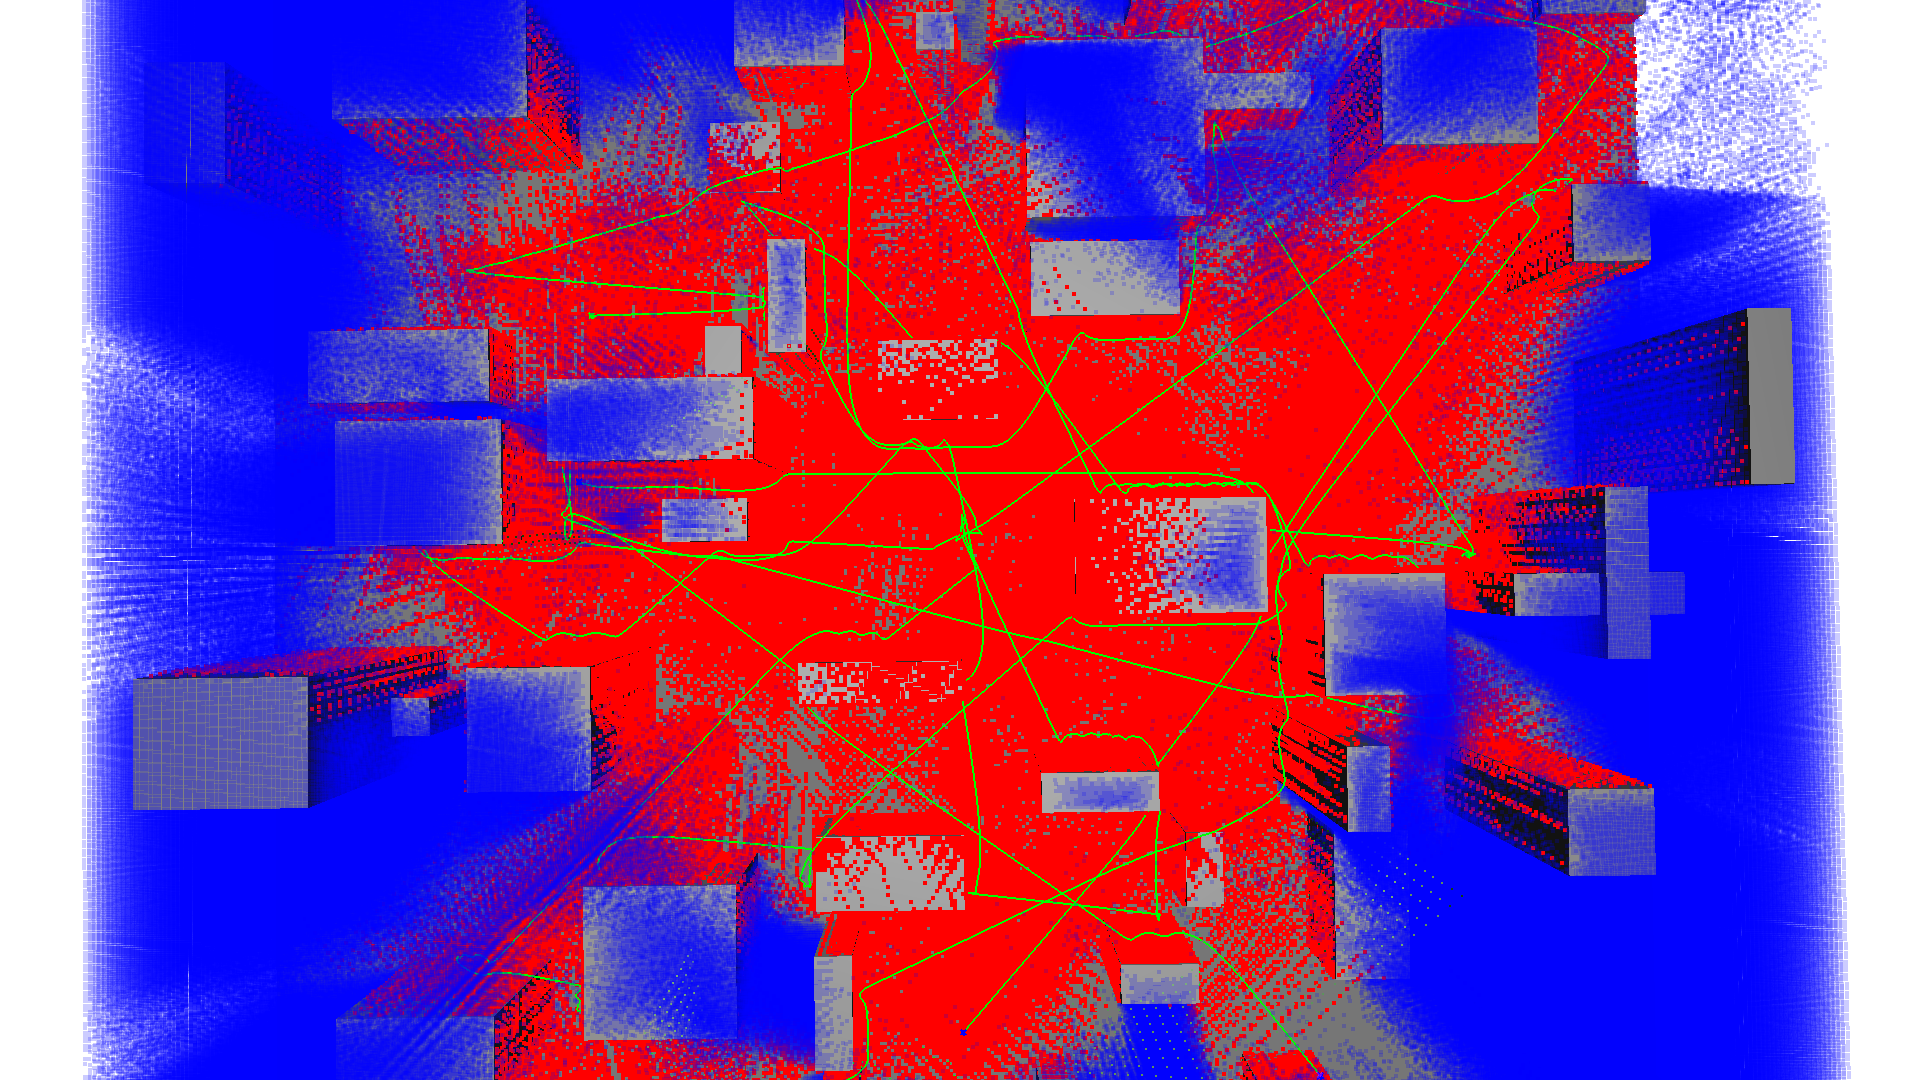
\includegraphics[width=\linewidth]{pa4.png}

Код проекта доступен по URL: \verb|https://github.com/deviator/dplm|.

???

\newpage
\subsection{Симуляция МБПЛА}

???

\newpage
\subsubsection{Модель карты местности}

На данном этапе выполнения работы было решено хранить информацию о местности в
виде дискретной карты с ограничениями по высоте, глубине и ширине. Карта
представляет из себя массив прямоугольных секторов, хранящих фиксированный объём
информации:
\begin{mintemize}
    \item факт обследованности
    \item наличие объекта
\end{mintemize}

Реализация карты представляет собой 1-мерный массив, к которому можно обратиться с помощью трёх
индексов-координат.

Правила перевода индекса в координаты и обратно:

\nextverbatimspread{1}
\begin{verbatim}
    z = index / ( width * height )
    tmp = index % ( width * height )
    y = tmp / width
    x = tmp % width

    index = z * width * height + y * width + x
\end{verbatim}
\vspace{-0.5em}

где:

\verb|a / b| -- целочисленное деление \verb|a| на \verb|b|;

\verb|a % b| -- остаток от деления \verb|a| на \verb|b|;

\verb|index| -- индекс в одномерном массиве;

\verb|width| -- ширина поля;

\verb|height| -- высота поля;

\verb|x,y,z| -- координаты по ширине, высоте и глубине соответственно.

Также для карты имеется матрица трансформации координат из локальных (индексов)
в глобальные (метры).

При разрешении карты $400 \times 400 \times 50$ получаем $8 \cdot 10^6$ секторов.
Обработку таких объёмов данных было решено производить с помощью гетерогенных 
вычислений на GPU. Была использована технология \verb|OpenCL|. Это так же 
позволяет решить вопрос отображения данных через \verb|OpenGL|, так как
интероперабельность с графической системой использует zero-copy память -- 
физически это один участок памяти для буферов \verb|OpenCL| и \verb|OpenGL|.

\newpage
\subsubsection{Модель единицы массива}

Примерный код функции $limit \left( \vec f \right)$:

\nextverbatimspread{1}
\begin{verbatim}
    vec3 limit( vec3 f )
    {
        if( f.xy.len > max_horisontal_force )
            f.xy = f.xy.e * max_horisontal_force;
        if( f.z > max_up_force ) f.z = max_up_force;
        if( f.z < min_up_force ) f.z = min_up_force;
        return f;
    }
\end{verbatim}

где:

\verb|f.xy| -- вектор, составленный из компонент вектора \verb|f|,

\verb|f.xy.len| -- длина вектора,

\verb|f.xy.e| -- единичный вектор.

Такой алгоритм обрезки максимальной тяги позволяет в горизонтальной плоскости двигаться к цели прямолинейно,
а выход на требуемую высоту происходит максимально быстро.

\newpage
\subsubsection{Модель измерителей и заполнение карты}

Предполагается что каждый юнит имеет возможность
оценить дальность в любом направлении, в нескольких точках одновременно с определённым 
угловым разрешением (карта глубин).

Каждый юнит получает информацю о мире с помощью датчика глубины в виде картинки,
где каждому пикселю соответствует измерение дальности в определённых угловых координатах. В работе не эмулировлись
дистрозийные искажения, поэтому для приведения карты глубин в точки в системе координат юнита достаточно 
матрицы перспективной трансформации, которая имеется у каждого юнита. Она также может меняться в процессе работы
системы при необходимости (изменение угла обзора, зум). Строится эта матрица так:

$$
M_{persp} = \left( \begin{array}{c c c c}
        \frac{1}{ R \cdot \tan( \frac{1}{2} A ) } & 0 & 0 & 0 \\
        0 & \frac{1}{ \tan( \frac{1}{2} A ) } & 0 & 0 \\
        0 & 0 & \frac{ z_{n} + z_{f} }{ z_{n}-z_{f} } & \frac{ 2 \cdot z_{n} \cdot z_{f} }{ z_{n} - z_{f} } \\
        0 & 0 & -1 & 0
\end{array} \right)
$$

где:

$R = \frac{w}{h}$ -- соотношение сторон изображения

$A$ -- угол обзора по вертикали

$z_{n}$ -- дальность от центра камеры до ближней плоскости отсечения

$z_{f}$ -- дальность от центра камеры до дальней плоскости отсечения

При трансформации точки с помощью перспективной матрицы координаты результирующей точки
получаются в диапазоне $x \in [-1,1]$, $y \in [-1,1]$, $z \in [0,1]$. Все точки, что выходят
за эти пределы, не отображаются. Для работы с четырёхменой матрицей необходимо использовать
однородные координаты.

Переход от однородных координат к декартовым: 

\verb|vec3 C = U.xyz / U.w|

Переход от декартовых к однородным:

\verb|vec4 U = vec4( C.xyz, 1 )|

где:

\verb|U| -- четырёхмерный вектор однородных координат,

\verb|C| -- трёхмерный вектор в декартовых координатах.

\newpage

Процесс получение карты глубин реализован посредством \verb|OpenGL|. Для этого 
производится рендеринг мира в Frame Buffer, где для карты глубин выставлена текстура, 
которая потом копируется в буфер \verb|OpenCL|. Копирование из текстуры в буфер реализованно
из-за ограничений \verb|OpenCL 1.1|. Прямое использование изображений с глубиной добавленно
только в стандарте \verb|OpenCL 2.0|, вышедшем в 2013г. Драйвер видеокарты на рабочей машине
не поддерживал последний стандарт.

Точки имеют дополнительную информацию -- было ли что-либо найдено.
Это вычисляется с так: \verb|bool finded = depth[iy*w+ix] < 1.0f - 1e-6;|.
То есть, если значение глубины крайне близко к максимальному, можно считать, что
луч из камеры не наткнулся ни на один объект.

После получения точек в связанной системе координат они приводятся
сначала к мировой, затем к системе координат карты.
Так же приводится положение юнита (камеры) к системе координат карты.

Заполняется карта по следующему алгоритму:
\begin{mintemize}
    \item строится отрезок из точки камеры (А) к точке, полученной с датчика (Б)
    \item все сектора, которые находятся между А и Б помечаются как исследованные
    \item сектор, в котором находится точка с датчика помечается как заполненый,
        если в ней было что-то найдено.
\end{mintemize}


